\documentclass[11pt,a4paper]{article}

\usepackage[T1]{fontenc}
\usepackage[margin=2.3cm]{geometry}
\usepackage{graphicx}
\usepackage{booktabs}
\usepackage{tabularx}
\usepackage{array}
\newcolumntype{Y}{>{\raggedright\arraybackslash}X}
\usepackage{longtable}
\usepackage{float}
\usepackage{caption}
\usepackage{amsmath}
\usepackage{enumitem}
\usepackage{listings}
\usepackage{fancyhdr}
\usepackage[hyphens]{url}
\usepackage[hidelinks]{hyperref}

\graphicspath{{../results/PartA/}{../results/PartD/}}

\lstset{basicstyle=\ttfamily\small, columns=fullflexible, keepspaces=true,
        frame=single, breaklines=true, showstringspaces=false}

\setlength{\parskip}{0.5em}
\setlength{\parindent}{0pt}
\renewcommand{\arraystretch}{1.15}
\newcommand{\um}{$\mu$m}
\newcommand{\umsq}{$\mu$m$^2$}
\newcommand{\cell}[1]{\texttt{#1}}

\pagestyle{fancy}
\fancyhf{}
\fancyhead[L]{Digital VLSI Design -- Assignment 1}
\fancyhead[R]{4-bit Array Multiplier: RTL to GDSII}
\fancyfoot[C]{\thepage}
\renewcommand{\headrulewidth}{0.4pt}
\setlength{\headheight}{14pt}
\setlength{\emergencystretch}{3em}

\begin{document}

% ------------------------------------------------------------------ title page
\thispagestyle{empty}
\begin{center}
\vspace*{5cm}
{\LARGE\bfseries Digital VLSI Design\par}
\vspace{0.4cm}
{\Large Assignment 1\par}
\vspace{1cm}
{\Large 4-bit Unsigned Array Multiplier from RTL to GDSII\par}
\vspace{0.3cm}
{SkyWater SKY130 (\texttt{sky130\_fd\_sc\_hd}) \,|\, Icarus Verilog, Yosys, OpenSTA, LibreLane\par}
\vspace{2cm}
\begin{tabular}{ll}
\toprule
\textbf{Team member} & \textbf{Roll number} \\
\midrule
Ande Karthik & 2023102009 \\
Kalluri Roshan Lal & 2023102010 \\
\bottomrule
\end{tabular}
\end{center}
\clearpage

% ------------------------------------------------------------------ contents
{\setlength{\parskip}{0pt}\small
\tableofcontents}
\clearpage

% ================================================================== 1
\section{Overview and Environment}

We designed a 4-bit $\times$ 4-bit unsigned array multiplier in Verilog, verified it with an exhaustive
self-checking testbench, synthesised it to SKY130 standard cells with Yosys, analysed its timing with
OpenSTA, and took it through place and route to a GDSII layout with LibreLane. The design registers its
inputs and its output, so every internal timing path runs from one flip-flop to another. The latency is
2 clock cycles and the throughput is one product per clock cycle.

\subsection{Tools and environment}

\begin{table}[H]
\centering
\begin{tabularx}{\textwidth}{lY}
\toprule
\textbf{Stage} & \textbf{Tool and version} \\
\midrule
RTL and gate-level simulation & Icarus Verilog 14.0 (\texttt{iverilog -g2012}, \texttt{vvp}) \\
Waveform viewing & GTKWave 4.0.0 \\
Logic synthesis & Yosys 0.70 with ABC \\
Static timing analysis & OpenSTA 3.1.0 \\
RTL-to-GDSII flow & LibreLane 3.1.0.dev3, Classic flow (Yosys, OpenROAD, Magic, KLayout, Netgen) \\
Layout viewing & KLayout with the SKY130 layer properties from the PDK \\
PDK and library & \texttt{sky130A}, \texttt{sky130\_fd\_sc\_hd}; Liberty file
                  \texttt{sky130\_fd\_sc\_hd\_\_tt\_025C\_1v80.lib} (typical corner) for Parts B and C \\
Environment & IIC-OSIC-TOOLS Docker image \texttt{hpretl/iic-osic-tools:latest} on Ubuntu 24.04.4;
              the project folder is mounted at \texttt{/foss/designs/mult4\_2023102009} \\
\bottomrule
\end{tabularx}
\caption{Tools used in each stage of the flow.}
\end{table}

The container's default PDK is IHP \texttt{ihp-sg13g2}, so SKY130 is selected explicitly in every step
(\texttt{\$PDK\_ROOT/sky130A/...} paths in Parts A--C and \texttt{PDK=sky130A} in Part D).

\subsection{Repository layout}

\begin{table}[H]
\centering
\begin{tabularx}{\textwidth}{lY}
\toprule
\textbf{Path} & \textbf{Contents} \\
\midrule
\texttt{README.md} & team, environment, every command in order \\
\texttt{rtl/full\_adder.v} & full adder (\texttt{assign} statements) \\
\texttt{rtl/mult\_array.v} & array multiplier: 16 AND gates, 12 \texttt{full\_adder} instances, 16 flip-flops \\
\texttt{tb/tb\_mult.v} & exhaustive self-checking testbench (256 vectors) \\
\texttt{synth/} & \texttt{synth.tcl} $\rightarrow$ \texttt{mult\_array\_netlist.v}, \texttt{mult\_array\_stat.rpt} \\
\texttt{sta/} & \texttt{sta.tcl} $\rightarrow$ \texttt{mult\_array\_timing.rpt} \\
\texttt{pnr/} & \texttt{config.json} $\rightarrow$ \texttt{metrics.json}, \texttt{mult\_array.gds} (final run) \\
\texttt{results/PartA..PartD/} & logs, tables, screenshots and write-ups for every task \\
\texttt{report/report.pdf} & this report \\
\bottomrule
\end{tabularx}
\caption{Repository layout.}
\end{table}

\clearpage
% ================================================================== 2
\section{Part A: RTL Design and Verification}

\subsection{Full adder}

\texttt{rtl/full\_adder.v} defines module \texttt{full\_adder} with inputs \texttt{a}, \texttt{b},
\texttt{cin} and outputs \texttt{sum}, \texttt{cout}, written only with \texttt{assign} statements:
\begin{align*}
\texttt{sum}  &= a \oplus b \oplus cin && \text{(1 when an odd number of inputs are 1)}\\
\texttt{cout} &= a\,b + b\,cin + a\,cin && \text{(majority: 1 when two or more inputs are 1)}
\end{align*}

\subsection{Array multiplier architecture}

For every bit $b_i$ of $B$ there is one partial product $pp_i = A \wedge b_i$, so
$pp_i[j] = a[j]\cdot b[i]$. This gives $4 \times 4 = 16$ AND gates. Row 0 has no adders. Rows 1 to 3 are
4-bit ripple-carry adders of 4 full adders each, giving $3 \times 4 = 12$ full adders. Each row adds its
partial product to the 4 bits passed down from the row above; the lowest sum bit of each row is a
finished product bit.

\begin{table}[H]
\centering
\resizebox{\textwidth}{!}{%
\begin{tabular}{clll}
\toprule
\textbf{Row} & \textbf{Inputs to full adder $j$} & \textbf{Outputs} \\
\midrule
0 & no adders (AND gates only) & $p[0] = pp_0[0]$;\; $r_0 = \{0, pp_0[3], pp_0[2], pp_0[1]\}$ \\
1 & $pp_1[j], r_0[j], c_1[j]$ \;($c_1[0]=0$) & $s_1[j], c_1[j{+}1]$;\; $p[1] = s_1[0]$;\; $r_1 = \{c_1[4], s_1[3], s_1[2], s_1[1]\}$ \\
2 & $pp_2[j], r_1[j], c_2[j]$ \;($c_2[0]=0$) & $s_2[j], c_2[j{+}1]$;\; $p[2] = s_2[0]$;\; $r_2 = \{c_2[4], s_2[3], s_2[2], s_2[1]\}$ \\
3 & $pp_3[j], r_2[j], c_3[j]$ \;($c_3[0]=0$) & $s_3[j], c_3[j{+}1]$;\; $p[3] = s_3[0]$;\; $p[7{:}4] = \{c_3[4], s_3[3], s_3[2], s_3[1]\}$ \\
\bottomrule
\end{tabular}}
\caption{Connections of the array (Section 2 of the assignment).}\label{tab:conn}
\end{table}

Implementation in \texttt{rtl/mult\_array.v}:
\begin{itemize}[nosep]
  \item Ports \texttt{clk}, \texttt{rst\_n} (asynchronous, active low), \texttt{a[3:0]}, \texttt{b[3:0]},
        \texttt{p[7:0]} (registered), exactly as specified.
  \item Input registers \texttt{a\_reg}, \texttt{b\_reg} (8 flip-flops) capture \texttt{a} and \texttt{b}
        on every rising edge; reset clears them to 0.
  \item Partial products \texttt{pp\textit{i} = a\_reg \& \{4\{b\_reg[\textit{i}]\}\}}: the 16 AND gates.
  \item Three adder rows with 4 \texttt{full\_adder} instances each (\texttt{fa10}..\texttt{fa33}),
        12 instances in total; carry chains \texttt{c1}, \texttt{c2}, \texttt{c3} with bit 0 tied to 0.
  \item The 8-bit result is registered into \texttt{p} (8 flip-flops), giving 16 flip-flops in total.
  \item The \texttt{*} operator is not used anywhere in the RTL.
\end{itemize}

\subsection{Block diagram}

\begin{figure}[H]
\centering
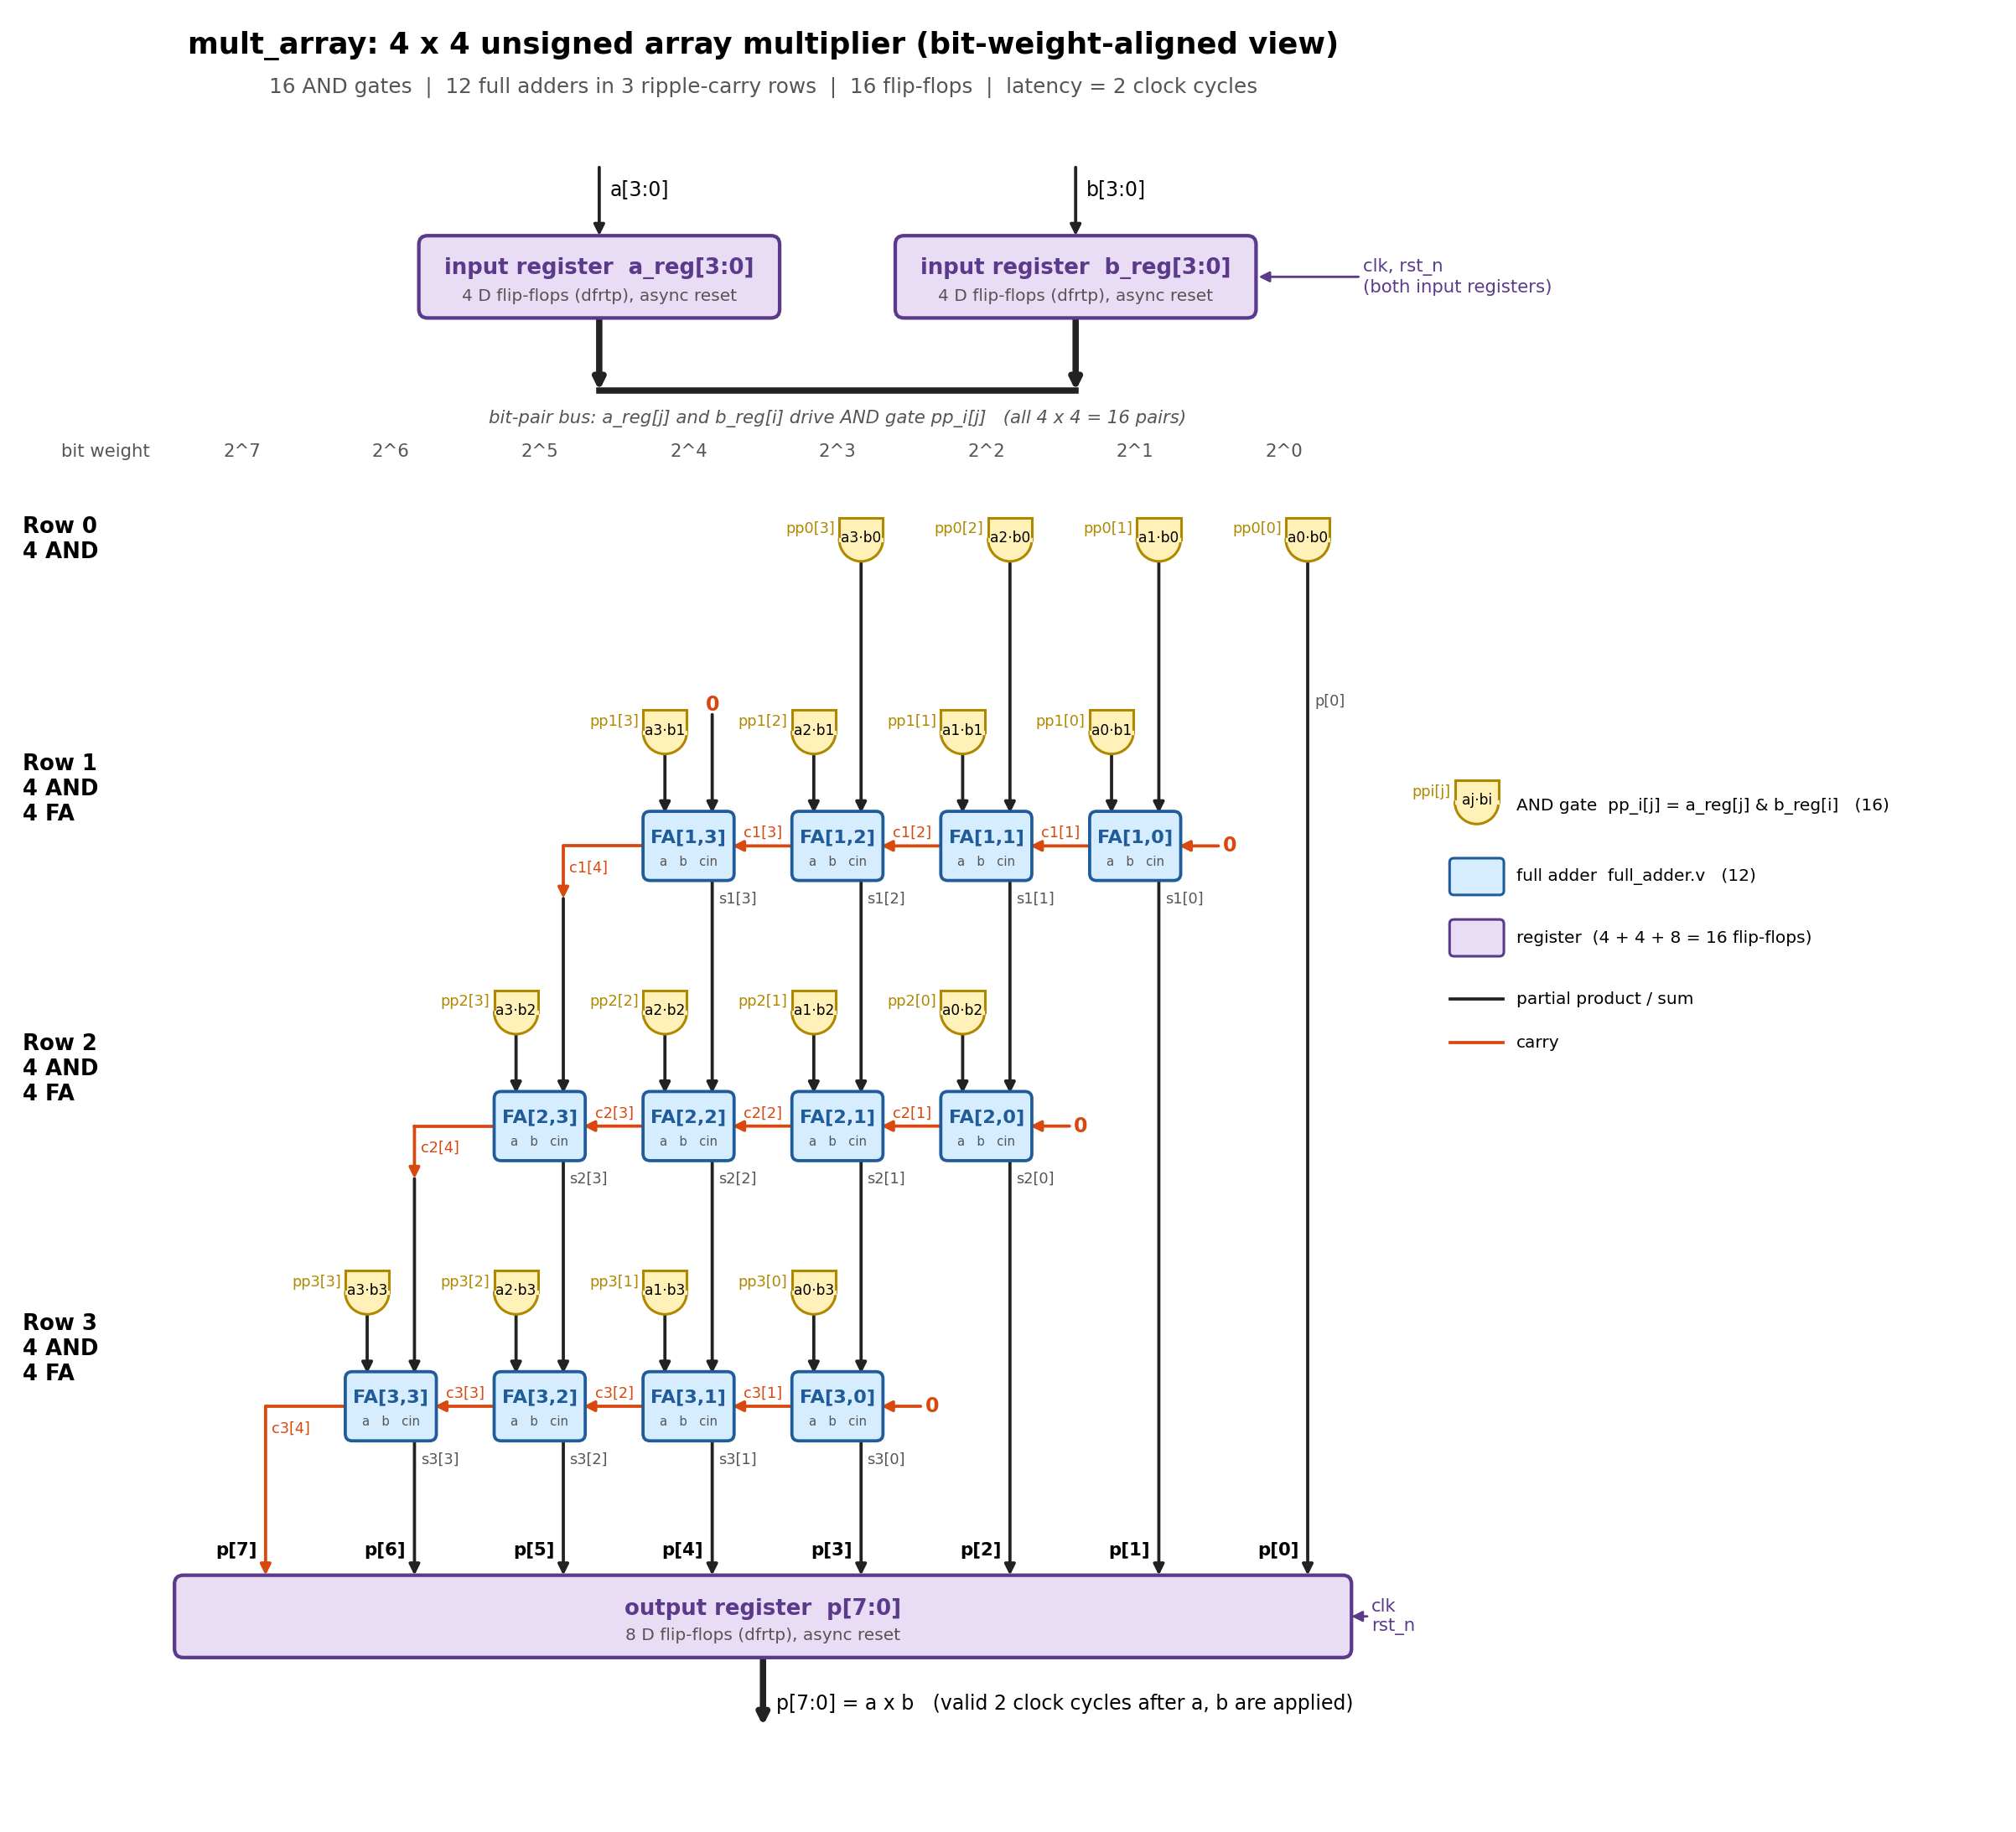
\includegraphics[width=\textwidth]{block_diagram.png}
\caption{Block diagram of \texttt{mult\_array} in a bit-weight-aligned layout: input registers
\texttt{a\_reg}/\texttt{b\_reg} (8 flip-flops), 16 AND gates $pp_i[j]$, 12 full adders FA[$i$,$j$] in three
ripple-carry rows, and the output register \texttt{p} (8 flip-flops). Partial products and sums flow
straight down, carries flow from right to left.}
\end{figure}

\subsection{Testbench}

\begin{table}[H]
\centering
\begin{tabularx}{\textwidth}{>{\raggedright\arraybackslash}p{4.6cm}Y}
\toprule
\textbf{Requirement} & \textbf{How \texttt{tb/tb\_mult.v} meets it} \\
\midrule
10 ns clock; \texttt{rst\_n} low for the first 2 cycles &
\texttt{always \#5 clk = \~{}clk}. \texttt{rst\_n} is 0 from time 0 and is released at the falling edge after
the second rising edge (20 ns). \\
All 256 input combinations & Nested loops \texttt{a\_value} = 0..15 and \texttt{b\_value} = 0..15. \\
Wait for the 2-cycle latency and compare with \texttt{a * b} &
Inputs change at a falling edge; the testbench waits two rising edges (capture into \texttt{a\_reg}/\texttt{b\_reg},
then into \texttt{p}) and checks \texttt{p} 2 ns later against \texttt{expected = a\_value * b\_value}.
The \texttt{*} operator appears only here. \\
Print every mismatch; one summary line &
\texttt{Mismatch: a=.. b=.. expected=.. got=..} for each error, then exactly one
\texttt{PASS: 256 vectors checked, 0 errors} or \texttt{FAIL: 256 vectors checked, N errors}. \\
Waveform file \texttt{mult.vcd} & \texttt{\$dumpfile("mult.vcd"); \$dumpvars(0, tb\_mult);} \\
\bottomrule
\end{tabularx}
\caption{Testbench requirements and how \texttt{tb/tb\_mult.v} meets them.}
\end{table}

Each vector takes 2 clock cycles (20 ns): vector $k$ is applied at $30 + 20k$ ns and checked 17 ns later,
so the last check is at $47 + 20 \times 255 = 5147$ ns, matching \texttt{\$finish called at 5147000 (1ps)}.

\subsection{Simulation results}

\begin{lstlisting}
$ iverilog -g2012 -o sim tb/tb_mult.v rtl/full_adder.v rtl/mult_array.v
$ vvp sim
VCD info: dumpfile mult.vcd opened for output.
PASS: 256 vectors checked, 0 errors
\end{lstlisting}

\textbf{Error-injection test (task 6).} To check that the testbench catches errors, the sum in
\texttt{full\_adder.v} was temporarily changed from \texttt{a \^{} b \^{} cin} to \texttt{a \^{} b},
which ignores the carry-in. The testbench was run again and the file was then restored with
\texttt{git checkout rtl/full\_adder.v} (\texttt{git diff} empty, PASS again):

\begin{lstlisting}
Mismatch: a=3 b=3 expected=9 got=5
Mismatch: a=3 b=6 expected=18 got=10
Mismatch: a=3 b=7 expected=21 got=9
Mismatch: a=3 b=11 expected=33 got=29
Mismatch: a=3 b=12 expected=36 got=20
... (90 more Mismatch lines)
FAIL: 256 vectors checked, 95 errors
\end{lstlisting}

95 of the 256 products are wrong. A vector can only fail when some full adder has a carry-in of 1, so
products that never create an internal carry (for example $a = 0$, $b = 0$ or a power-of-two operand)
still pass. The testbench therefore detects a broken adder. Logs: \texttt{results/PartA/1\_rtl\_sim\_pass.log},
\texttt{results/PartA/2\_fail\_test.log}.

\subsection{Hand-worked example (task 5)}

Roll number 2023102009 (last digit 9): $A = 9 + 5 = 14 = 1110_2$, $B = 7 = 0111_2$ ($A \neq 7$, so $B$ stays 7).
The expected product is $14 \times 7 = 98 = 0110\,0010_2$.

\begin{minipage}{\linewidth}
\begin{lstlisting}
          1 1 1 0     A  = 14
        x 0 1 1 1     B  =  7
  -----------------
          1 1 1 0     pp0 = A AND b0 (b0 = 1)              = 14
        1 1 1 0       pp1 = A AND b1 (b1 = 1), shifted 1   = 28
      1 1 1 0         pp2 = A AND b2 (b2 = 1), shifted 2   = 56
    0 0 0 0           pp3 = A AND b3 (b3 = 0), shifted 3   =  0
  -----------------
    0 1 1 0 0 0 1 0   P = 14 + 28 + 56 + 0 = 98
\end{lstlisting}
\end{minipage}

The same product through the adder rows of Table~\ref{tab:conn} (bits written MSB first):

\begin{table}[H]
\centering
\begin{tabular}{ccccl}
\toprule
\textbf{Row} & $pp_i$ & $r_{i-1}$ & $\{c_i[4], s_i\}$ & \textbf{Outputs} \\
\midrule
0 & 1110 & -- & -- & $p[0] = 0$, $r_0 = 0111$ \\
1 & 1110 & 0111 & 1\,0101 (14 + 7 = 21) & $p[1] = 1$, $r_1 = 1010$ \\
2 & 1110 & 1010 & 1\,1000 (14 + 10 = 24) & $p[2] = 0$, $r_2 = 1100$ \\
3 & 0000 & 1100 & 0\,1100 (0 + 12 = 12) & $p[3] = 0$, $p[7{:}4] = 0110$ \\
\bottomrule
\end{tabular}
\caption{Row-by-row evaluation of $14 \times 7$ in the array.}
\end{table}

$P = \{p[7{:}4], p[3], p[2], p[1], p[0]\} = \{0110, 0, 0, 1, 0\} = 0110\,0010_2 = 98$, the same as the
shift-and-add result. The full working, including every full adder's inputs and outputs, is in
\texttt{results/PartA/hand\_example.txt}.

\subsection{Waveform}

In the exhaustive testbench the pair $a = 14$, $b = 7$ is vector $14 \times 16 + 7 = 231$, applied at
$30 + 20 \times 231 = 4650$ ns.

\begin{figure}[H]
\centering
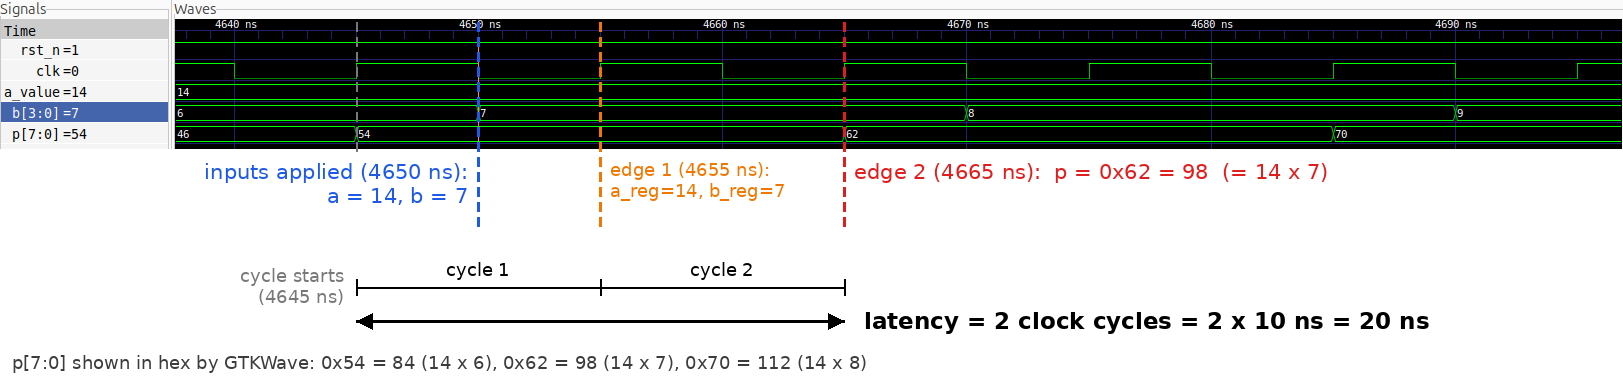
\includegraphics[width=\textwidth]{latency_marking.png}
\caption{GTKWave view of \texttt{clk}, \texttt{rst\_n}, the input values (\texttt{a\_value} is the testbench
variable that drives \texttt{a}), \texttt{b} and \texttt{p} for $A = 14$, $B = 7$. The inputs are applied at
4650 ns, captured into the input registers at rising edge 1 (4655 ns), and the product
\texttt{0x62} = 98 appears on \texttt{p} at rising edge 2 (4665 ns): the latency is 2 clock cycles (20 ns).
GTKWave shows \texttt{p} in hexadecimal (\texttt{0x54} = 84, \texttt{0x62} = 98, \texttt{0x70} = 112).}
\end{figure}

\clearpage
% ================================================================== 3
\section{Part B: Logic Synthesis with Yosys}

\subsection{Synthesis script}

\begin{table}[H]
\centering
\begin{tabularx}{\textwidth}{c>{\raggedright\arraybackslash}p{7.4cm}Y}
\toprule
\textbf{Step} & \textbf{Command in \texttt{synth/synth.tcl}} & \textbf{Purpose} \\
\midrule
1 & \texttt{yosys read\_verilog rtl/full\_adder.v rtl/mult\_array.v} & Read the design \\
2 & \texttt{yosys synth -top mult\_array -flatten} & Generic synthesis; flatten the 12 full adders \\
3 & \texttt{yosys dfflibmap -liberty \$lib} & Map flip-flops to SKY130 cells \\
4 & \texttt{yosys abc -liberty \$lib} & Map the logic to SKY130 gates \\
5 & \texttt{yosys opt\_clean -purge} & Remove unused wires \\
6 & \texttt{yosys tee -o synth/mult\_array\_stat.rpt stat -liberty \$lib} & Cell and area report \\
7 & \texttt{yosys write\_verilog -noattr synth/mult\_array\_netlist.v} & Gate-level netlist \\
\bottomrule
\end{tabularx}
\caption{Steps of \texttt{synth/synth.tcl}, run with \texttt{yosys -c synth/synth.tcl}.}
\end{table}

\texttt{\$lib} is the typical-corner Liberty file
\path{$PDK_ROOT/sky130A/libs.ref/sky130_fd_sc_hd/lib/sky130_fd_sc_hd__tt_025C_1v80.lib}.

\subsection{Part B results}

\begin{table}[H]
\centering
\begin{tabularx}{\textwidth}{lY}
\toprule
\textbf{Metric} & \textbf{Value} \\
\midrule
Total number of cells & 73 \\
Number of flip-flops & 16 (\cell{sky130\_fd\_sc\_hd\_\_dfrtp\_1}: D flip-flop with active-low asynchronous reset) \\
Total cell area (\umsq) & 805.77 \\
Flip-flop area (\umsq) & 400.38 = 16 $\times$ 25.024 \\
Flip-flop area (\% of total) & 49.69 \% \\
The 3 most-used cell types and their counts & \cell{dfrtp\_1} $\times$ 16, \cell{nand2\_1} $\times$ 11, \cell{a21oi\_1} $\times$ 4 \\
Netlist simulation result & \texttt{PASS: 256 vectors checked, 0 errors} \\
\bottomrule
\end{tabularx}
\caption{Part B results table (from \texttt{synth/mult\_array\_stat.rpt}).}
\end{table}

\subsection{Full cell breakdown}

\begin{table}[H]
\centering
\small
\begin{tabular}{>{\raggedright\arraybackslash}p{3.5cm}>{\raggedright\arraybackslash}p{8.0cm}rr}
\toprule
\textbf{Group} & \textbf{Cells (\texttt{sky130\_fd\_sc\_hd\_\_...})} & \textbf{Count} & \textbf{Area (\umsq)} \\
\midrule
Flip-flops & \cell{dfrtp\_1} $\times$16 & 16 & 400.384 \\
Sum logic (XOR/XNOR) & \cell{xnor2\_1} $\times$4, \cell{xnor3\_1} $\times$2, \cell{xor3\_1} $\times$1 & 7 & 103.850 \\
Carry logic (majority) & \cell{maj3\_1} $\times$1 & 1 & 10.010 \\
AND gates & \cell{and2\_0} $\times$4, \cell{and3\_1} $\times$1, \cell{and4\_1} $\times$1 & 6 & 40.038 \\
NAND / NOR & \cell{nand2\_1} $\times$11, \cell{nand3\_1}, \cell{nand4\_1} $\times$4, \cell{nor2\_1}, \cell{nor2b\_1}, \cell{nor3\_1} & 19 & 86.334 \\
AND-OR / OR-AND compound & \cell{a21oi\_1} $\times$4, \cell{a21boi\_0} $\times$2, \cell{o21ai\_0} $\times$2, \cell{o31a\_1} $\times$2, \cell{a21o\_1}, \cell{a22oi\_1}, \cell{a32oi\_1}, \cell{o2111a\_1}, \cell{o2111ai\_1}, \cell{o21a\_1}, \cell{o22ai\_1}, \cell{o311ai\_0}, \cell{o31ai\_1}, \cell{or3\_1} & 20 & 148.651 \\
Isolation-type cells & \cell{lpflow\_inputiso1p\_1}, \cell{lpflow\_isobufsrc\_1} $\times$2 & 3 & 18.768 \\
Inverters & \cell{clkinv\_1} & 1 & 3.754 \\
\midrule
\textbf{Total (31 cell types)} & & \textbf{73} & \textbf{805.773} \\
\bottomrule
\end{tabular}
\caption{All cells in the synthesised netlist, grouped by function (cells without a count appear once).}\label{tab:cells}
\end{table}

\subsection{Gate-level (netlist) simulation}

The synthesised netlist was simulated with the same testbench and the SKY130 cell models, to show that
synthesis did not change the behaviour:

\begin{lstlisting}
$ CELLS=$PDK_ROOT/sky130A/libs.ref/sky130_fd_sc_hd/verilog
$ iverilog -g2012 -DFUNCTIONAL -DUNIT_DELAY=#1 -o gls \
    tb/tb_mult.v $CELLS/primitives.v $CELLS/sky130_fd_sc_hd.v synth/mult_array_netlist.v
$ vvp gls
VCD info: dumpfile mult.vcd opened for output.
PASS: 256 vectors checked, 0 errors
tb/tb_mult.v:73: $finish called at 5147000 (1ps)
\end{lstlisting}

\clearpage
% ================================================================== 4
\section{Part C: Static Timing Analysis with OpenSTA}

\subsection{STA script and constraints}

\begin{table}[H]
\centering
\begin{tabularx}{\textwidth}{c>{\raggedright\arraybackslash}p{8.2cm}Y}
\toprule
\textbf{Step} & \textbf{Command in \texttt{sta/sta.tcl}} & \textbf{Purpose} \\
\midrule
1 & \texttt{read\_liberty \$lib} (tt\_025C\_1v80) & Read the cell timing library \\
2 & \texttt{read\_verilog synth/mult\_array\_netlist.v}; \texttt{link\_design mult\_array} & Read and link the netlist \\
3 & \texttt{create\_clock -name clk -period \$clock\_period [get\_ports clk]} & Clock with period $T$ (10 ns, or \texttt{STA\_PERIOD}) \\
4 & \texttt{set\_input\_delay 1.0 -clock clk [delete\_from\_list [all\_inputs] [get\_ports clk]]} & Input arrival time \\
5 & \texttt{set\_output\_delay 1.0 -clock clk [all\_outputs]} & Output required time \\
6 & \texttt{report\_worst\_slack -max} & Worst setup slack \\
7 & \texttt{report\_checks -path\_delay max -digits 3 > sta/mult\_array\_timing.rpt} & Critical path report \\
\bottomrule
\end{tabularx}
\caption{Steps of \texttt{sta/sta.tcl}, run with \texttt{sta -exit sta/sta.tcl}.}
\end{table}

The analysis is pre-layout: the clock is ideal (no skew or insertion delay) and there is no wire delay.

\subsection{Finding the maximum frequency}

\begin{lstlisting}
$ sta -exit sta/sta.tcl                    (T = 10.00 ns)
worst slack max 7.40                       (report: +7.404 ns)

T_min = T - WNS   = 10.000 - 7.404 = 2.596 ns
F_max = 1000/T_min = 1000 / 2.596   = 385.21 MHz

$ STA_PERIOD=2.60 sta -exit sta/sta.tcl    (T = T_min rounded to 0.01 ns)
worst slack max 0.00                       (report: +0.004 ns)
\end{lstlisting}

At $T = 2.60$ ns the slack is +0.004 ns, effectively zero, which confirms $T_{min}$. The small positive
value comes from rounding 2.596 ns up to 2.60 ns.

\subsection{Part C results}

\begin{table}[H]
\centering
\begin{tabularx}{\textwidth}{lY}
\toprule
\textbf{Metric} & \textbf{Value} \\
\midrule
Worst slack at $T$ = 10 ns (ns) & +7.404 \\
$T_{min}$ (ns) & 2.596 \\
$F_{max}$ (MHz) & 385.21 \\
Slack at $T = T_{min}$ (ns) & +0.004 at $T$ = 2.60 ns ($\approx 0$) \\
Critical path start point & \texttt{\_118\_}: input register \texttt{b\_reg[0]} (\cell{dfrtp\_1}, CLK$\rightarrow$Q) \\
Critical path end point & \texttt{\_112\_}: output register \texttt{p[6]} (\cell{dfrtp\_1}, D = \texttt{fa33.sum}) \\
Number of cells on the critical path & 10: 2 flip-flops + 8 combinational cells \\
Latency (ns) = $2 \times T_{min}$ & 5.192 \\
Throughput (million results per second) & 385.21 (one result per clock cycle) \\
\bottomrule
\end{tabularx}
\caption{Part C results table (typical corner, pre-layout).}
\end{table}

\subsection{Critical path}

\begin{table}[H]
\centering
\small
\resizebox{\textwidth}{!}{%
\begin{tabular}{rlllrr}
\toprule
\textbf{\#} & \textbf{Instance} & \textbf{Cell} & \textbf{Function in the multiplier} & \textbf{Incr (ns)} & \textbf{Arrival (ns)} \\
\midrule
1 & \texttt{\_118\_/Q} & \cell{dfrtp\_1} & input register \texttt{b\_reg[0]}, CLK$\rightarrow$Q & 0.395 & 0.395 \\
2 & \texttt{\_083\_/X} & \cell{and2\_0} & AND gate $pp_0[0] = a\_reg[0] \cdot b\_reg[0]$ & 0.212 & 0.607 \\
3 & \texttt{\_055\_/X} & \cell{or3\_1} & row-1 carry logic (merged) & 0.361 & 0.968 \\
4 & \texttt{\_059\_/X} & \cell{and4\_1} & row-1 carry logic merged with an \texttt{a\_reg[1]} AND & 0.215 & 1.183 \\
5 & \texttt{\_070\_/X} & \cell{o2111a\_1} & carry logic merged with $pp_2[2]$ & 0.234 & 1.417 \\
6 & \texttt{\_076\_/Y} & \cell{o21ai\_0} & carry-chain logic & 0.216 & 1.634 \\
7 & \texttt{\_090\_/X} & \cell{xnor3\_1} & full-adder sum & 0.274 & 1.907 \\
8 & \texttt{\_091\_/X} & \cell{maj3\_1} & full-adder carry & 0.375 & 2.282 \\
9 & \texttt{\_092\_/X} & \cell{xor3\_1} & full-adder sum of FA[3,3] $\rightarrow$ \texttt{fa33.sum} & 0.178 & 2.460 \\
10 & \texttt{\_112\_/D} & \cell{dfrtp\_1} & output register \texttt{p[6]}, setup 0.135 ns & 0.000 & 2.460 \\
\bottomrule
\end{tabular}}
\caption{Critical path from \texttt{sta/mult\_array\_timing.rpt} ($T$ = 2.60 ns). Cell roles were traced in
\texttt{synth/mult\_array\_netlist.v}.}
\end{table}

Data arrival = 2.460 ns; data required = 2.600 $-$ 0.135 = 2.465 ns; slack = +0.004 ns. At $T$ = 10 ns the same
path has slack 9.865 $-$ 2.460 = +7.404 ns. The input-to-register and register-to-output paths are short,
so the register-to-register path through the adder array sets $T_{min}$. The report also lists the
asynchronous reset recovery check (\texttt{rst\_n} $\rightarrow$ \texttt{RESET\_B}); its slack is +9.228 ns
at 10 ns and +1.828 ns at 2.60 ns, so it never limits the clock.

\subsection{Comparison with the $2N = 8$ full-adder estimate}

\begin{itemize}[nosep]
  \item The path has 8 combinational cells with 2.065 ns of logic delay ($2.460 - 0.395$), about 0.26 ns per cell.
  \item 7 of the 8 cells come from full-adder logic: 3 pure full-adder functions (\cell{xnor3} sum,
        \cell{maj3} carry, \cell{xor3} sum of FA[3,3]) and 4 compound gates (\cell{or3}, \cell{and4},
        \cell{o2111a}, \cell{o21ai}) that implement the ripple carry merged with partial-product ANDs.
        Only \cell{\_083\_} (\cell{and2\_0}) is a plain AND gate.
  \item This matches the estimate of about $2N = 8$ full-adder delays well. The match is approximate
        because \texttt{synth -flatten} removes the \texttt{full\_adder} boundaries and ABC folds AND gates
        and parts of several full adders into single compound cells.
\end{itemize}

\clearpage
% ================================================================== 5
\section{Part D: Physical Design with LibreLane}

\subsection{Configuration and flow}

LibreLane 3.1.0.dev3 (Classic flow) was run inside the IIC-OSIC-TOOLS container with the SKY130 PDK
selected (\texttt{export PDK=sky130A STD\_CELL\_LIBRARY=sky130\_fd\_sc\_hd}; \texttt{librelane config.json}).
The flow runs synthesis (Yosys), floorplan and power grid, tap insertion, placement, clock-tree synthesis
and timing repair, routing (OpenROAD), RC extraction and multi-corner STA, DRC (Magic and KLayout),
LVS (Netgen), and writes the GDSII.

\begin{lstlisting}[caption={\texttt{pnr/config.json} (final run)}]
{
  "DESIGN_NAME": "mult_array",
  "VERILOG_FILES": ["dir::../rtl/full_adder.v", "dir::../rtl/mult_array.v"],
  "CLOCK_PORT": "clk",
  "CLOCK_PERIOD": 7.0,
  "FP_SIZING": "absolute",
  "DIE_AREA": [0, 0, 150, 150]
}
\end{lstlisting}

The die is fixed at 150 \um{} $\times$ 150 \um{}. The core box is (5.52, 10.88) to (144.44, 138.72) \um{},
which holds 47 rows of \texttt{unithd} sites.

\subsection{Timing closure: every attempt}

Starting period: $1.2 \times T_{min} = 1.2 \times 2.596 = 3.115$ ns, rounded up to the next 0.5 ns = 3.5 ns.
After each run that failed setup timing, CLOCK\_PERIOD was increased by 0.5 ns. The configuration and
metrics of every attempt are kept in \texttt{results/PartD/attempts/}.

\begin{table}[H]
\centering
\resizebox{\textwidth}{!}{%
\begin{tabular}{cccccccc}
\toprule
\textbf{Run} & \textbf{Period (ns)} & \textbf{Setup slack (ns)} & \textbf{tt slack (ns)} & \textbf{Hold slack (ns)} & \textbf{DRC} & \textbf{LVS} & \textbf{Result} \\
\midrule
1 & 3.5 & $-2.154$ & +0.587 & +0.100 & 0 & 0 & FAIL (setup) \\
2 & 4.0 & $-1.654$ & +1.087 & +0.147 & 0 & 0 & FAIL (setup) \\
3 & 4.5 & $-1.154$ & +1.587 & +0.147 & 0 & 0 & FAIL (setup) \\
4 & 5.0 & $-0.654$ & +2.087 & +0.147 & 0 & 0 & FAIL (setup) \\
5 & 5.5 & $-0.155$ & +2.587 & +0.147 & 0 & 0 & FAIL (setup) \\
6 & 6.0 & $-0.107$ & +2.899 & +0.148 & 0 & 0 & FAIL (setup) \\
7 & 6.5 & $-0.136$ & +3.199 & +0.141 & 0 & 0 & FAIL (setup) \\
8 & \textbf{7.0} & \textbf{+0.364} & +3.699 & +0.141 & 0 & 0 & \textbf{PASS} \\
\bottomrule
\end{tabular}}
\caption{All LibreLane runs. Setup slack = \texttt{setup\_\_ws}, the worst over all 9 signoff corners (always
the slow corner \texttt{ss\_100C\_1v60}); tt slack = typical corner \texttt{nom\_tt\_025C\_1v80}.}
\end{table}

From 3.5 ns to 5.5 ns the slack improves by exactly 0.5 ns per step, as expected when only the period
changes. At 6.0 ns and 6.5 ns it improves very little and even gets worse. The synthesised netlist was
identical in all 8 runs, so the change comes from the place-and-route timing repair choosing a different
critical path. The typical corner passed in every run; only the slow corner limited the period.

\subsection{Part D results}

\begin{table}[H]
\centering
\begin{tabularx}{\textwidth}{lY}
\toprule
\textbf{Metric} & \textbf{Value} \\
\midrule
CLOCK\_PERIOD used (ns) & 7.0 \\
Number of runs needed & 8 (3.5 $\rightarrow$ 7.0 ns in 0.5 ns steps) \\
Core area (\umsq) & 17759.5 (die area 22500 = 150 $\times$ 150 \um) \\
Cells after synthesis (from Part B) & 73 (16 flip-flops + 57 logic cells) \\
Cells after place and route & 1895 instances (334 excluding decap/fill) \\
Kinds of cells added & buffers $\times$22 (\cell{buf\_2}, \cell{clkdlybuf4s50\_1}, \cell{clkbuf\_16}),
                       tap $\times$245 (\cell{tapvpwrvgnd\_1}), decap $\times$1314 (\cell{decap\_*}),
                       fill $\times$247 (\cell{fill\_*}) \\
Wirelength (\um) & 2362 (552 vias) \\
Setup slack (ns) & +0.364 (worst corner \texttt{max\_ss\_100C\_1v60}) \\
Post-route $F_{max}$ (MHz) & 150.70 = 1000 / (7.0 $-$ 0.364) \\
$F_{max}$ from Part C (MHz) & 385.21 \\
DRC errors & 0 (Magic 0, KLayout 0, router 0) \\
LVS errors & 0 (Netgen: circuits match uniquely) \\
\bottomrule
\end{tabularx}
\caption{Part D results table (final run, CLOCK\_PERIOD = 7.0 ns, from \texttt{pnr/metrics.json}).}
\end{table}

\subsection{Timing at every signoff corner}

\begin{table}[H]
\centering
\resizebox{\textwidth}{!}{%
\begin{tabular}{llrrr}
\toprule
\textbf{Corner (process, V, T)} & \textbf{Wire RC} & \textbf{Setup slack (ns)} & \textbf{Hold slack (ns)} & \textbf{Implied $F_{max}$ (MHz)} \\
\midrule
tt, 1.80 V, 25 $^\circ$C   & min & 3.729 & 0.363 & 305.7 \\
                           & nom & 3.699 & 0.370 & 302.9 \\
                           & max & 3.678 & 0.374 & 301.1 \\
\midrule
ss, 1.60 V, 100 $^\circ$C  & min & 0.444 & 0.822 & 152.5 \\
                           & nom & 0.406 & 0.815 & 151.7 \\
                           & max & \textbf{0.364} & 0.808 & \textbf{150.7} \\
\midrule
ff, 1.95 V, $-40$ $^\circ$C & min & 4.735 & 0.141 & 441.6 \\
                           & nom & 4.726 & 0.145 & 439.8 \\
                           & max & 4.719 & 0.148 & 438.5 \\
\bottomrule
\end{tabular}}
\caption{Setup and hold slack at each of the 9 signoff corners (final run). Implied $F_{max}$ = 1000 / (7.0 $-$ setup slack).}
\end{table}

The worst setup path is register-to-register (\texttt{timing\_\_setup\_r2r\_\_ws} = 0.364 ns), from
\texttt{\_102\_} (\texttt{a\_reg[0]}) to \texttt{\_100\_} (D = \texttt{fa33.sum}, output \texttt{p[6]}): the
same output bit as the Part C path. Setup clock skew is 0.26--0.28 ns at every corner. Other signoff
numbers: 0 antenna violations, 0 max-slew / max-capacitance / max-fanout violations, 0 disconnected pins,
worst IR drop 0.77 mV, total power 0.335 mW.

\subsection{Post-route $F_{max}$ compared with Part C}

Post-route $F_{max} = 1000/(7.0 - 0.364) = 150.70$ MHz, about 2.6 times lower than the 385.21 MHz of
Part C. Two effects combine:
\begin{enumerate}[nosep]
  \item \textbf{Corner} (about $2\times$). Part C used only the typical corner, while \texttt{setup\_\_ws} is set
        by the slow corner (1.60 V, 100 $^\circ$C), where the cells are about twice as slow. The same layout at
        the typical corner gives $1000/(7.0 - 3.699) = 302.9$ MHz.
  \item \textbf{Physical effects} (about 27 \% at the same corner). The minimum period at the typical corner
        grows from 2.596 ns to 3.301 ns (Table~\ref{tab:fmaxbreak}).
\end{enumerate}

\begin{table}[H]
\centering
\small
\begin{tabular}{>{\raggedright\arraybackslash}p{5.0cm}cc>{\raggedright\arraybackslash}p{4.2cm}}
\toprule
\textbf{Component} & \textbf{Part C (ns)} & \textbf{Post-route, tt (ns)} & \textbf{Added (ns)} \\
\midrule
Launch flip-flop CLK$\rightarrow$Q & 0.395 & 0.472 & +0.077 (real wire load) \\
Logic cells + wires & 2.065 (8 cells) & 2.439 (9 cells) & +0.374 (wire RC, LibreLane's netlist) \\
Clock uncertainty & 0 & 0.250 & +0.250 (LibreLane default) \\
Clock skew (0.336 $-$ 0.302 $-$ CRPR 0.018) & 0 & 0.016 & +0.016 \\
Library setup time & 0.135 & 0.124 & $-$0.011 \\
\midrule
\textbf{Minimum period} & \textbf{2.596} & \textbf{3.301} & \textbf{+0.705} \\
\bottomrule
\end{tabular}
\caption{Where the extra delay comes from at the typical corner (post-route report of path
\texttt{a\_reg[0]} $\rightarrow$ \texttt{p[6]}).}\label{tab:fmaxbreak}
\end{table}

\subsection{Cells added by place and route}

Part B synthesis gave \textbf{73 cells}; after place and route there are \textbf{1895 cells}
(\path{design__instance__count}), about 26 times more. The added cells were found by name in the
LibreLane cell-frequency report:

\begin{table}[H]
\centering
\small
\begin{tabularx}{\textwidth}{l>{\raggedright\arraybackslash}p{5.4cm}rY}
\toprule
\textbf{Name contains} & \textbf{Cells} & \textbf{Count} & \textbf{Why the flow adds them} \\
\midrule
\texttt{buf} & \cell{buf\_2} $\times$17, \cell{clkdlybuf4s50\_1} $\times$2 & 19 & Timing repair: drive long nets and fix slew, setup and hold. \\
             & \cell{clkbuf\_16} $\times$3 & 3 & Clock-tree synthesis: deliver the clock to the 16 flip-flops with low skew. \\
\texttt{tap} & \cell{tapvpwrvgnd\_1} & 245 & Tie the n-well to VPWR and the substrate to VGND at regular intervals to prevent latch-up. \\
\texttt{decap} & \cell{decap\_3} $\times$130, \cell{decap\_4} $\times$49, \cell{decap\_6} $\times$175, \cell{decap\_8} $\times$55, \cell{decap\_12} $\times$905 & 1314 & Decoupling capacitors between VPWR and VGND that reduce supply noise and IR drop. \\
\texttt{fill} & \cell{fill\_1} $\times$215, \cell{fill\_2} $\times$32 & 247 & Close the gaps so every row is continuous (wells, implants, power rails) and density rules are met. \\
\midrule
\multicolumn{2}{l}{\textbf{Added in total}} & \textbf{1828} & \\
\multicolumn{2}{l}{Logic (51) + flip-flops (16), from LibreLane's own synthesis} & 67 & \\
\multicolumn{2}{l}{\textbf{Total after place and route}} & \textbf{1895} & \\
\bottomrule
\end{tabularx}
\caption{Instance classes in the final layout.}\label{tab:added}
\end{table}

The logic part is 67 cells rather than Part B's 73 because LibreLane runs its own Yosys synthesis with a
different script; $67 + 1828 = 1895$. Without decap and fill cells there are 334 standard-cell instances with
an area of 1224.92 \umsq, a utilisation of only 6.9 \% of the 17759.5 \umsq{} core. The fixed
150 \um{} $\times$ 150 \um{} die is much larger than this design needs, which is why tap, decap and fill
cells make up almost all of the instances.

\subsection{Final layout}

\begin{figure}[H]
\centering
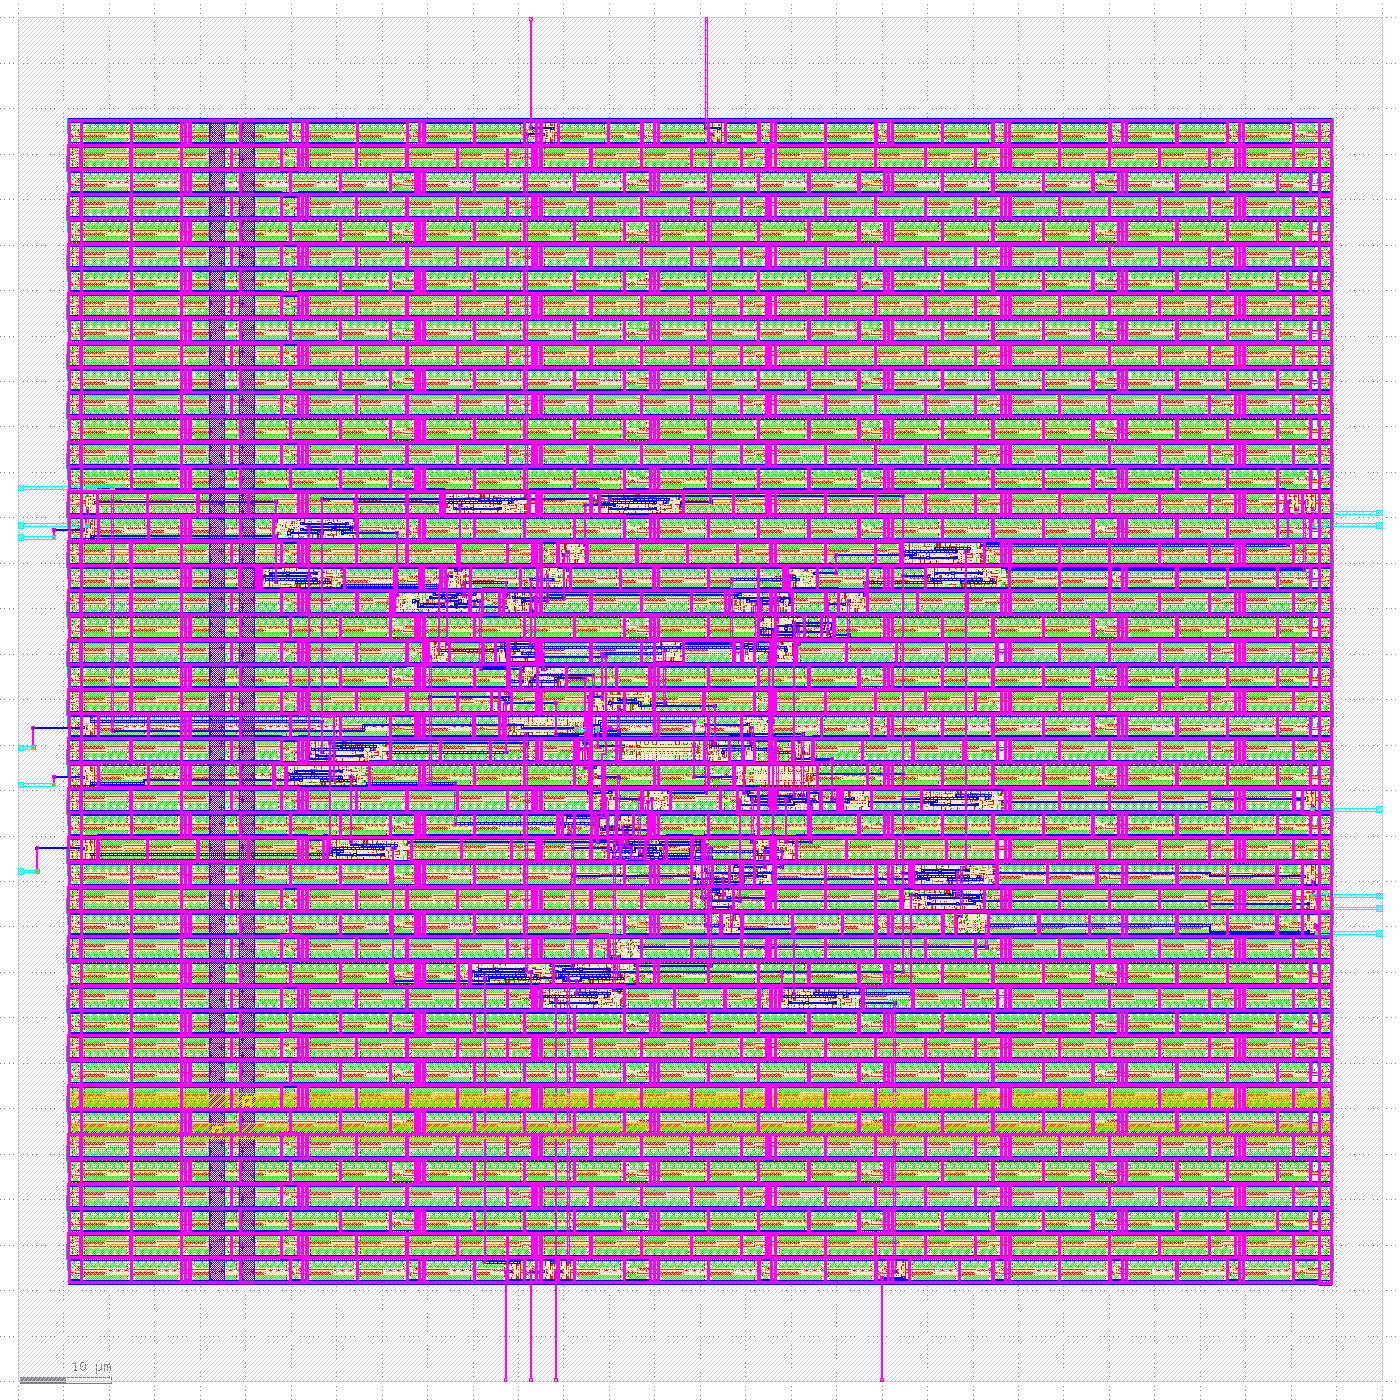
\includegraphics[width=0.8\textwidth]{layout_whole_die.png}
\caption{Whole die (150 \um{} $\times$ 150 \um) in KLayout: I/O pins on the die edges, 47 standard-cell rows
with the power grid, and the routed logic in the centre of the core.}
\end{figure}

\begin{figure}[H]
\centering
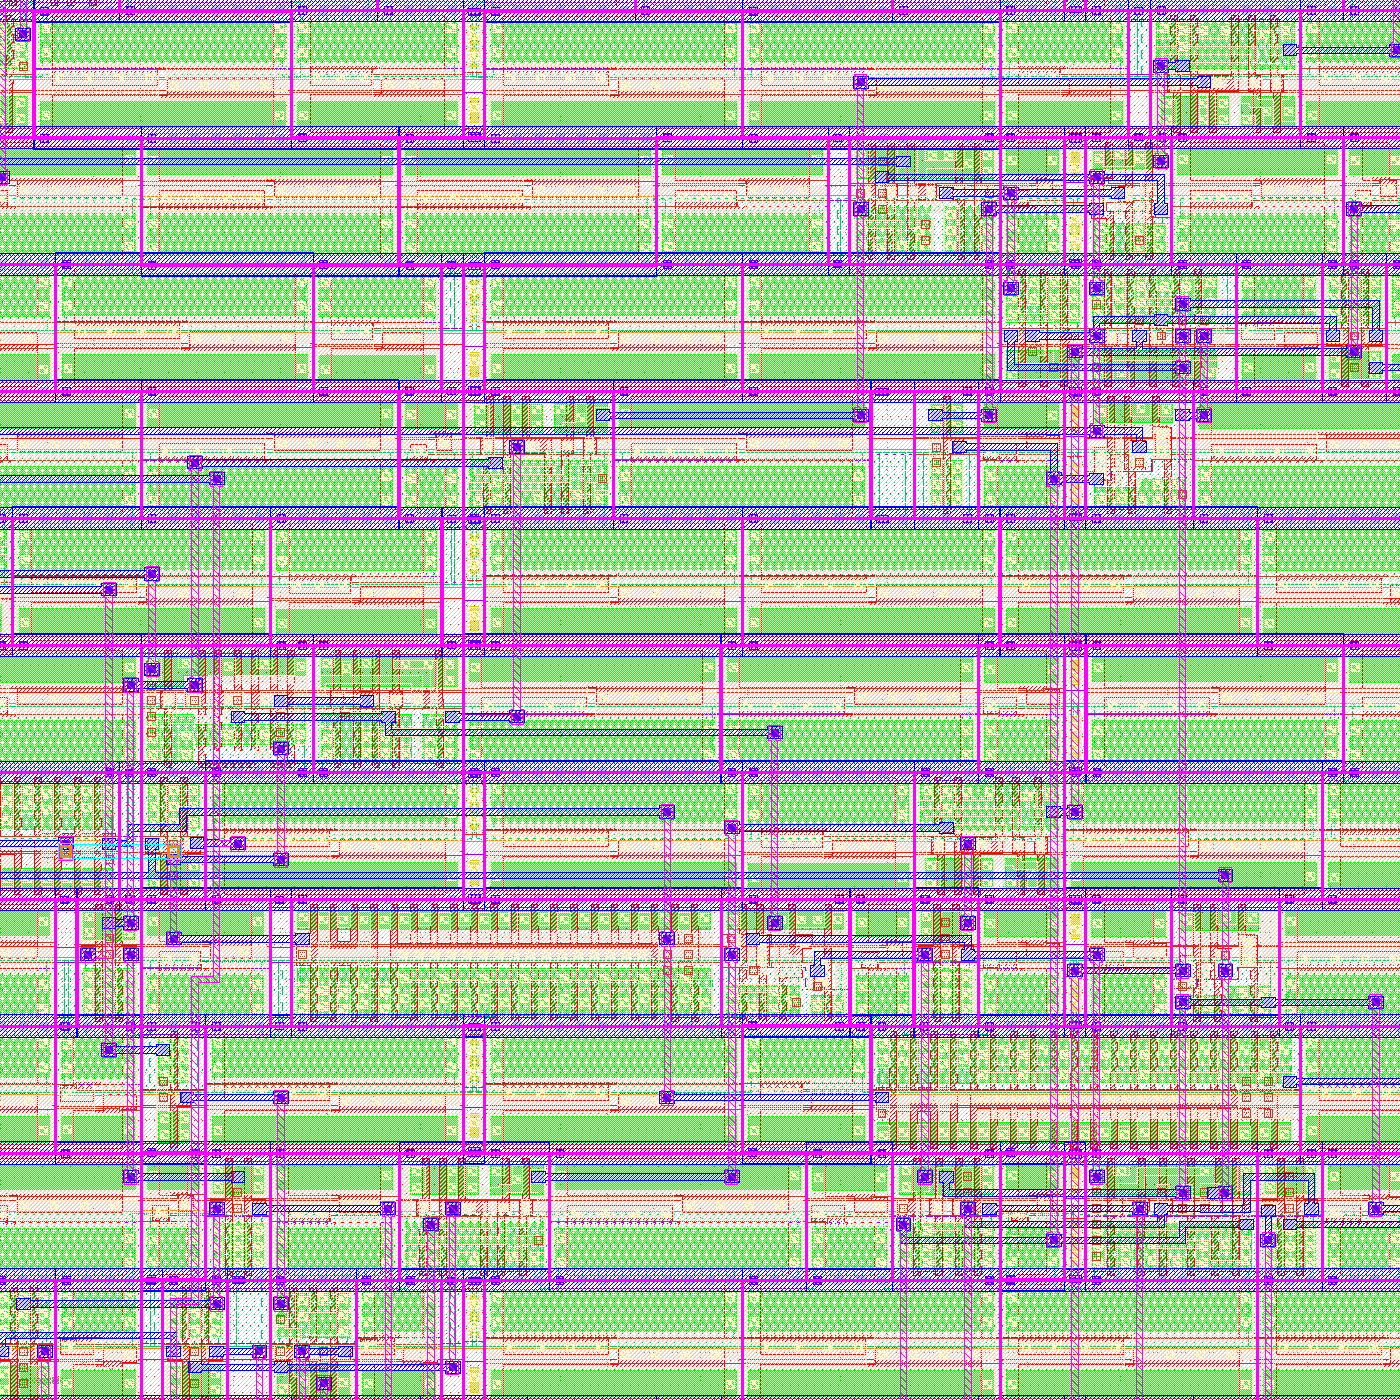
\includegraphics[width=0.75\textwidth]{layout_zoom.png}
\caption{Zoomed view (30 \um{} $\times$ 30 \um): standard-cell rows bounded by the horizontal power rails, with
routed metal-1/metal-2 wires and vias connecting the cell pins.}
\end{figure}

\begin{figure}[H]
\centering
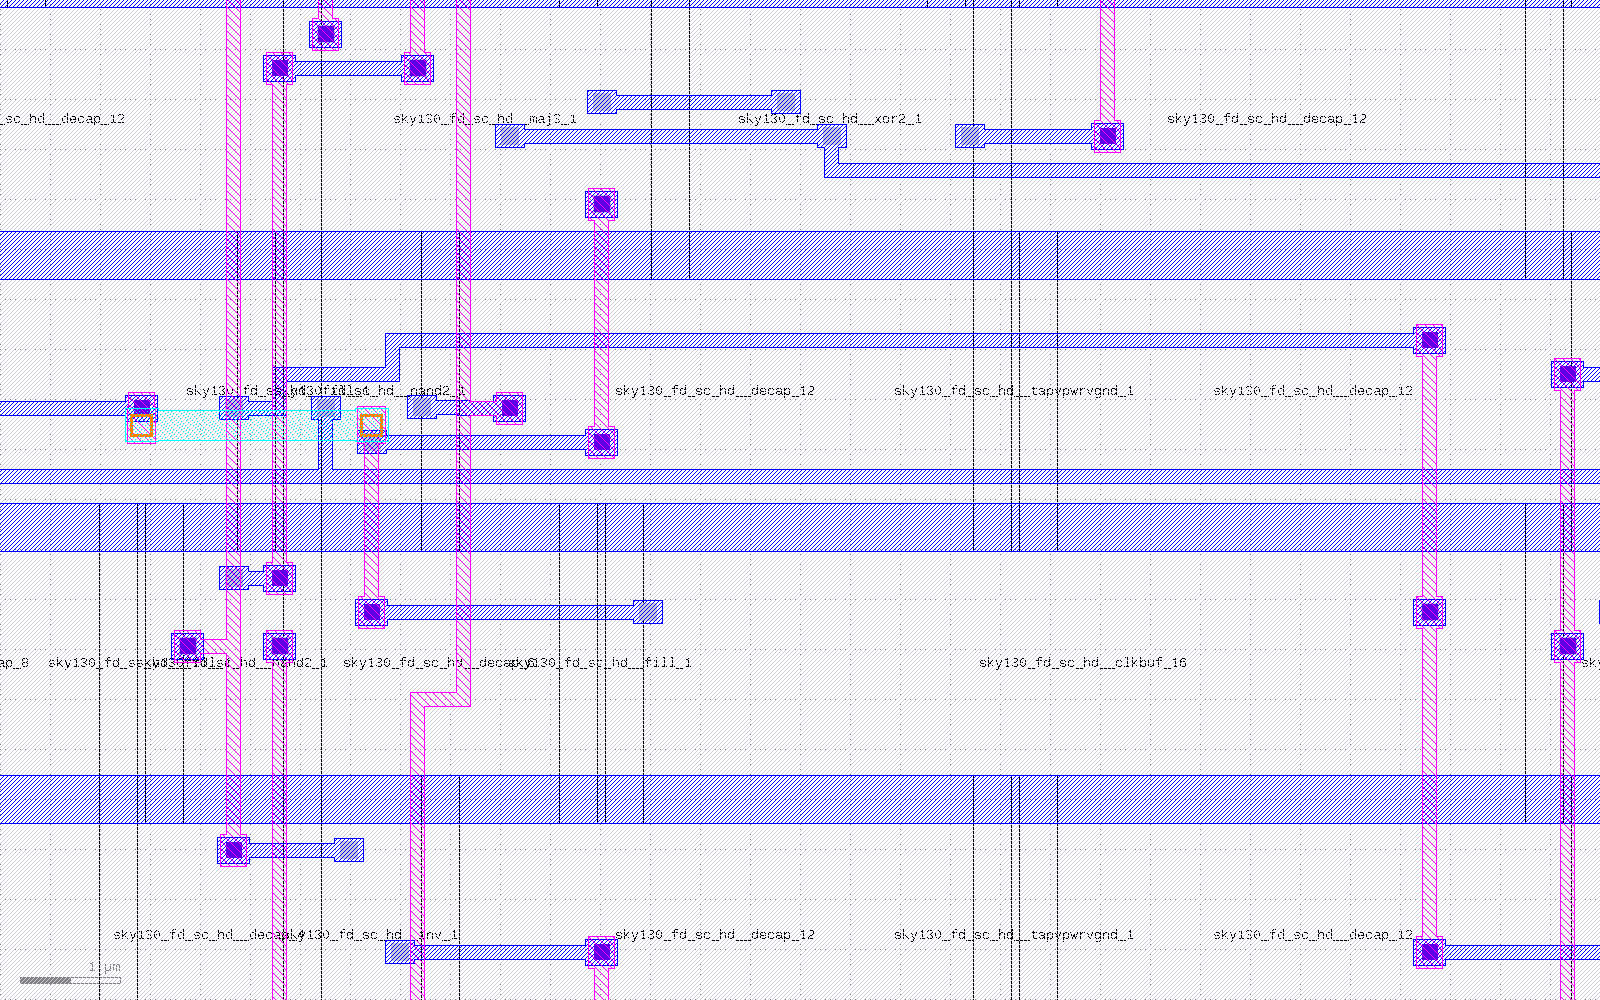
\includegraphics[width=\textwidth]{layout_zoom_cells.png}
\caption{Deeper zoom (16 \um{} $\times$ 10 \um) with every standard cell drawn as a labelled box: logic cells
(\cell{maj3\_1}, \cell{xor2\_1}, \cell{nand2\_1}, \cell{inv\_1}) next to cells added by the flow
(\cell{decap\_12}, \cell{tapvpwrvgnd\_1}, \cell{fill\_1}, \cell{clkbuf\_16}), the power rails between rows
and the routed wires.}
\end{figure}

\clearpage
% ================================================================== 6
\section{Answers to the Report Questions}

\subsection*{Q1. The array needs 16 AND gates and 12 full adders. How many cells did synthesis produce for the logic? Explain why the number of cells is not simply 16 + 12.}
\addcontentsline{toc}{subsection}{Q1. Logic cell count}

Synthesis produced 73 cells, of which 16 are flip-flops, so the logic uses \textbf{57 cells}
(405.39 \umsq) rather than 28. An ``AND gate'' and a ``full adder'' are RTL building blocks, not one library
cell each. With \texttt{-flatten}, Yosys removes the \texttt{full\_adder} boundaries, and ABC re-implements
the whole Boolean function with whichever SKY130 cells give a good area/delay result (Table~\ref{tab:cells}):
\begin{itemize}[nosep]
  \item \textbf{A full adder needs at least two cells.} Its sum becomes an XOR/XNOR cell (\cell{xnor2},
        \cell{xnor3}, \cell{xor3}; 7 in total) and its carry a \cell{maj3} or an equivalent NAND/AOI network.
        ABC cannot use the two-output SKY130 full-adder cell \cell{fa\_1} (the log reports ``Detected 9
        multi-output cells''), so 12 full adders alone need about 24 or more cells.
  \item \textbf{AND gates are merged into other logic.} Most partial-product ANDs are absorbed into compound
        gates such as \cell{a21oi}, \cell{a21boi}, \cell{o2111a}, \cell{nand4}; only 6 remain as plain
        \cell{and2/3/4} cells.
  \item \textbf{Constant inputs simplify some adders.} Every row's carry-in and the top bit of $r_0$ are 0,
        so those full adders reduce to half adders built from fewer, simpler gates.
\end{itemize}
The exact count depends on the RTL style and the tool version (ABC is a heuristic), but it is always well
above 28.

\subsection*{Q2. What is the critical path of your design, from which register to which register? How many cells are on it, and how does this compare with the estimate of about 2N full-adder delays?}
\addcontentsline{toc}{subsection}{Q2. Critical path}

The critical path starts at the input register \texttt{b\_reg[0]} (\texttt{\_118\_}, \cell{dfrtp\_1}) and ends
at the output register \texttt{p[6]} (\texttt{\_112\_}, \cell{dfrtp\_1}), whose D input is the sum of the last
full adder FA[3,3]. It has \textbf{10 cells}: the launching flip-flop, 8 combinational cells
(\cell{and2} $\rightarrow$ \cell{or3} $\rightarrow$ \cell{and4} $\rightarrow$ \cell{o2111a} $\rightarrow$
\cell{o21ai} $\rightarrow$ \cell{xnor3} $\rightarrow$ \cell{maj3} $\rightarrow$ \cell{xor3}) and the capturing
flip-flop. The data arrives at 2.460 ns, giving $T_{min}$ = 2.596 ns. The path follows the carry through the
adder rows into product bit 6. For $N = 4$ the estimate is $2N = 8$ full-adder delays, which matches the 8
combinational cells; 7 of them come from full-adder logic and the average delay is about 0.26 ns per cell.

\subsection*{Q3. What percentage of the total cell area is flip-flops? Why is this percentage large for such a small design?}
\addcontentsline{toc}{subsection}{Q3. Flip-flop area}

Flip-flops take 400.38 of 805.77 \umsq{} = \textbf{49.69 \%} of the cell area, although they are only 16 of the
73 cells (22 \%). One \cell{dfrtp\_1} is 25.02 \umsq: 6.7 times a \cell{nand2\_1} (3.75 \umsq), about 3.5 times
the average logic cell (7.1 \umsq), and larger than the biggest logic cell in the design (\cell{xor3\_1},
23.77 \umsq). An edge-triggered flip-flop with asynchronous reset is two latches plus clock and reset
circuitry, a few dozen transistors compared with 4 for a NAND2. The second reason is scaling: the array
logic grows as $N^2$ (16 ANDs, 12 adders), while the registers grow only as $4N$ (16 flip-flops). At
$N = 4$ the logic is still small, so the registers dominate; at 8 bits the flip-flop share falls to about
32 \% (Q6).

\subsection*{Q4. Why is the post-route F\textsubscript{max} lower than the F\textsubscript{max} from Part C? Which kinds of cells did the flow add, and why is each kind needed?}
\addcontentsline{toc}{subsection}{Q4. Post-route Fmax and added cells}

The post-route $F_{max}$ is 150.70 MHz against 385.21 MHz from Part C, about 2.6 times lower:
\begin{enumerate}[nosep]
  \item \textbf{Corner.} Part C used only the typical library (tt, 1.80 V, 25 $^\circ$C). LibreLane signs off at
        9 corners and reports the worst, the slow corner (ss, 1.60 V, 100 $^\circ$C, maximum wire RC). The same
        layout allows 302.9 MHz at the typical corner, so the corner accounts for about a factor of 2.
  \item \textbf{Real wires.} Part C had no parasitics. After routing, 2362 \um{} of wire and 552 vias add
        resistance and capacitance; the logic delay on the critical path grows by 0.374 ns and CLK$\rightarrow$Q by 0.077 ns.
  \item \textbf{Real clock.} Part C used an ideal clock. The routed design has a clock tree with skew and
        LibreLane's 0.25 ns clock uncertainty, which reduce the time available for setup.
  \item \textbf{Different netlist.} LibreLane re-synthesises the RTL with its own script, so the post-route
        critical path (\texttt{a\_reg[0]} $\rightarrow$ \texttt{p[6]}, 9 logic cells) is not the same as in Part C.
\end{enumerate}
At the same (typical) corner these physical effects add 0.705 ns to the minimum period (Table~\ref{tab:fmaxbreak}).

The flow added these cells (Table~\ref{tab:added}):
\begin{itemize}[nosep]
  \item \textbf{Buffers (22)}: \cell{buf\_2}, \cell{clkdlybuf4s50\_1} (timing repair: long nets, slew, setup,
        hold) and \cell{clkbuf\_16} (clock tree: low-skew clock to the 16 flip-flops).
  \item \textbf{Tap cells (245)}: bias the n-well and substrate to prevent latch-up.
  \item \textbf{Decap cells (1314)}: on-chip supply decoupling against switching noise.
  \item \textbf{Fill cells (247)}: keep the wells, implants and power rails continuous across row gaps so the
        layout passes DRC.
\end{itemize}

\subsection*{Q5. What does a DRC check verify, and what does an LVS check verify? Why must both pass before a chip can be manufactured?}
\addcontentsline{toc}{subsection}{Q5. DRC and LVS}

\textbf{DRC} (design rule check) verifies the geometry of the layout against the foundry's rules for every
layer: minimum widths, spacings, enclosures, overlaps, via rules, density and antenna ratios. These rules
describe what the fab can print reliably; a violation can cause shorts, opens or very low yield.

\textbf{LVS} (layout versus schematic) extracts the transistors and their connections from the layout and
compares them with the intended netlist: the same devices, nets and pins. It confirms that the layout is
the circuit we designed, with no missing connection, accidental short or swapped pin.

Each check covers what the other cannot. A layout can be manufacturable (DRC clean) but implement the wrong
circuit, or be the right circuit (LVS clean) but impossible to fabricate. A mask set is very expensive and
cannot be fixed after tape-out, so both must pass first. Our final run has 0 DRC errors in Magic and
KLayout (the router's intermediate violations, 28 $\rightarrow$ 3 $\rightarrow$ 3 $\rightarrow$ 0, were all fixed),
0 LVS errors in Netgen (``Circuits match uniquely'') and 0 antenna violations.

\subsection*{Q6. Using the formulas in Section 2, estimate how the number of full adders and the critical path delay would change if the multiplier were 8 bits wide instead of 4. Show your working.}
\addcontentsline{toc}{subsection}{Q6. Scaling to 8 bits}

\begin{table}[H]
\centering
\begin{tabular}{llccc}
\toprule
\textbf{Quantity} & \textbf{Formula} & \textbf{N = 4 (ours)} & \textbf{N = 8 (estimate)} & \textbf{Change} \\
\midrule
AND gates & $N^2$ & 16 & 64 & $\times 4$ \\
Full adders & $N(N-1)$ & 12 & 56 & $\times 4.67$ \\
Flip-flops & $2N + 2N$ & 16 & 32 & $\times 2$ \\
Critical path & $\approx 2N$ full-adder delays & 8 & 16 & $\times 2$ \\
\bottomrule
\end{tabular}
\caption{Scaling from 4 to 8 bits.}
\end{table}

\textbf{Working.} In Part C the 8 full-adder delays take 2.065 ns of logic, so one full-adder delay is about
$2.065/8 \approx 0.258$ ns. The flip-flop overhead is 0.395 (CLK$\rightarrow$Q) + 0.135 (setup) = 0.530 ns.
For $N = 8$:
\begin{align*}
T_{min}(8\text{-bit}) &\approx 0.530 + 16 \times 0.258 = 0.530 + 4.13 \approx 4.66 \text{ ns}\\
F_{max}(8\text{-bit}) &\approx 1000 / 4.66 \approx 215 \text{ MHz} \quad (\text{vs } 385 \text{ MHz for 4 bits; typical corner, pre-layout})
\end{align*}
The number of full adders grows about 4.7 times (quadratically in $N$), while the critical path grows only
about 2 times in its logic part (linearly in $N$). $T_{min}$ rises from 2.60 ns to about 4.66 ns, 1.8 times,
because the flip-flop overhead stays the same. For area, scaling the logic by the number of building blocks,
$(64 + 56)/(16 + 12) \approx 4.3$ times 405 \umsq{} gives about 1740 \umsq; with 32 flip-flops
(801 \umsq) the total is about 2540 \umsq{} and the flip-flop share falls to about 32 \%.

\end{document}
